\problemname{}

\illustration{0.2}{fish.png}{
    CC BY-SA 4.0 by ChatGPT
}


Vous êtes un explorateur marin, vous avez fait une découverte dans les profondeurs de l'océan là où la lumière du soleil ne peut plus atteindre, une étrange espèce de poisson bioluminescent, connue sous le nom de Karwa.

Ces poissons ont une particularitée assez spéciale, ils ont des écailles réfléchissantes qui réfléchissent la lumière dans des directions précises.

Vous décidez donc d'en apprendre un peu plus sur cette espèce de poisson, plus particulièrement leurs position. En effet il semblerait qu'il y ait un certain pattern dans leurs position.

Pour se faire, vous avez enregistré la position de tous les karwa aux alentours mais le problème c'est qu'il y a plusieurs bandes de karwa au même endroit. Votre but est de déterminer combiens de karwa font parti d'une bande étant donné un poisson spécifique.

Vous avez remarqué que 2 karwa font parti de la même bande si en envoyant de la lumière sur un des karwa, la lumière est réfléchie sur l'autre karwa.

Hereusement, vous avez aussi enregistré dans quel direction chaque karwa réfléchi la lumière. Cette direction est exprimée en degré et étonnament c'est toujour un nombre entier.

\smallskip
\begin{figure}[h]
    \centering
    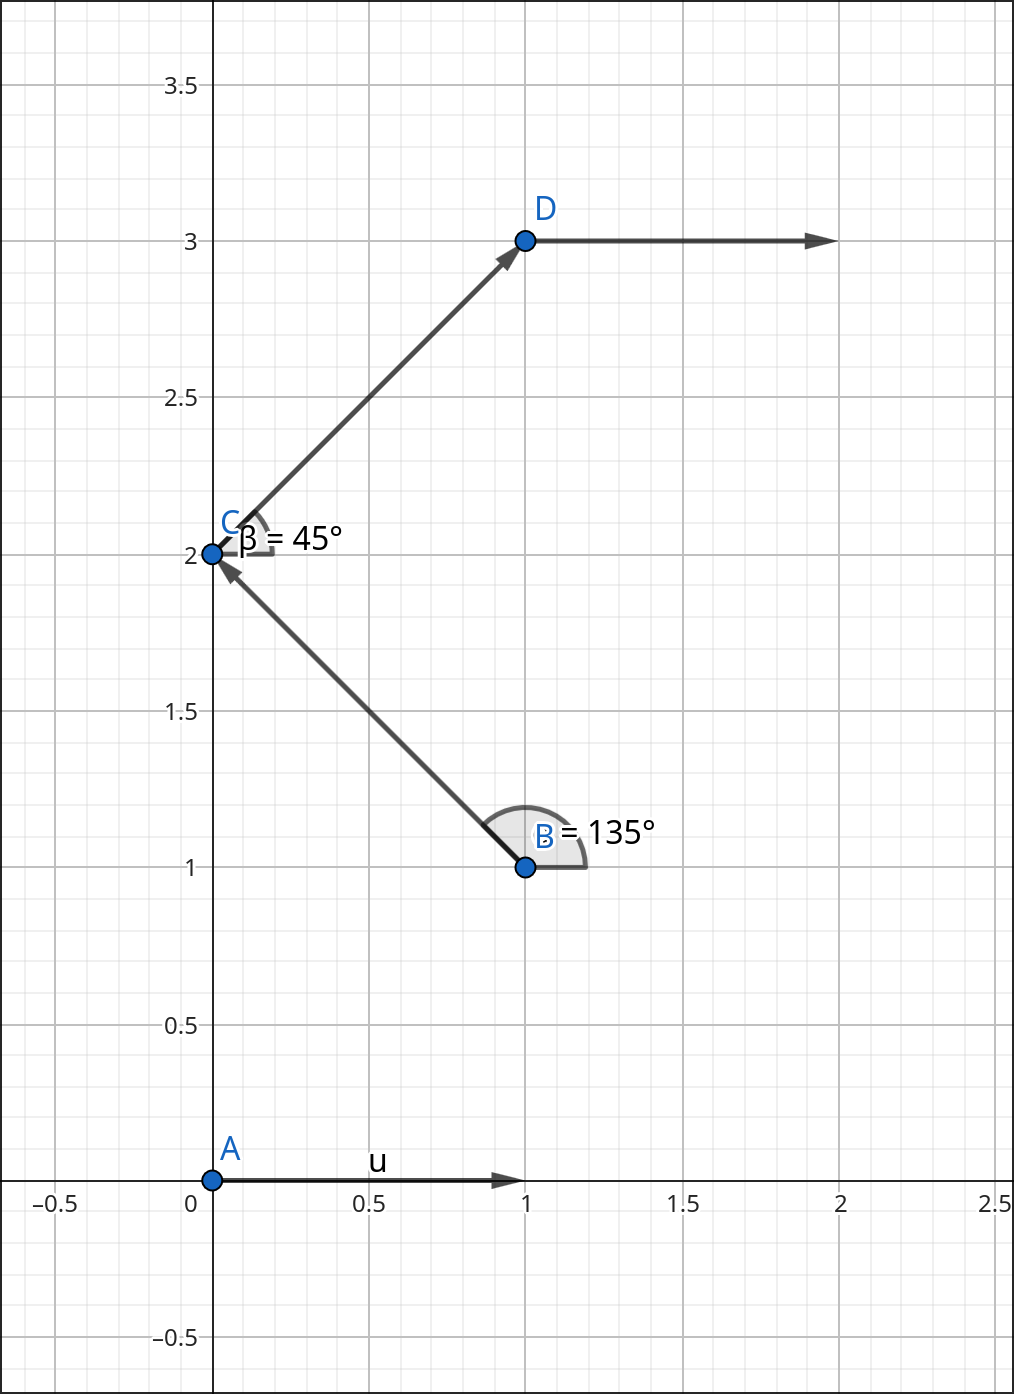
\includegraphics[width=0.3\textwidth]{sample1.png}
    \caption{Example du sample 1}
\end{figure}

\begin{Input}
    L'entrée consiste en:
    \begin{itemize}
        \item une ligne avec un entier $n$ ($0\leq n\leq 10^{5}$), le nombre de poisson.
        \item $n$ lignes avec $2$ nombre RÉEL $x, y$ ($-10^{18} \leq x,y \leq {10^{18}}$) et un entier d, ($0 \leq d \leq 360$). Qui sont respectivement l'emplacement du poisson ainsi que la direction dans laquel ils réfléchissent la lumière.
        \item une ligne avec un entier $a$ ($0 \leq a, b \leq n$) qui est le poisson que vous analysez.
    \end{itemize}
\end{Input}

\begin{Output}
    La taille de la bande.
\end{Output}
